% Generated by AP Math GOLD PILOT deterministic Python generator.
% input id: 02_coordinate_parallel
\documentclass{article}
\usepackage[margin=1cm]{geometry}
\def\pgfsysdriver{pgfsys-dvisvgm.def}
\usepackage{amssymb}
\usepackage{pgfplots}
\pgfplotsset{compat=1.18}
\pagestyle{empty}
\begin{document}
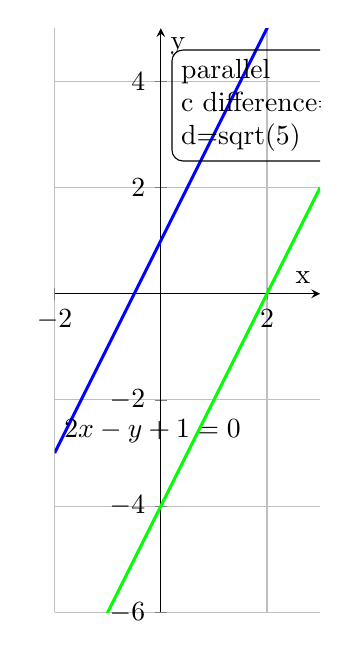
\begin{tikzpicture}
\begin{axis}[width=13cm,height=9cm,axis equal image,axis lines=middle,grid=major,xmin=-2,xmax=3,ymin=-6,ymax=5,xlabel={x},ylabel={y},clip=true]
\addplot[blue, solid, line width=1.1pt] coordinates {(-2,-3) (-1.9375,-2.875) (-1.875,-2.75) (-1.8125,-2.625) (-1.75,-2.5) (-1.6875,-2.375) (-1.625,-2.25) (-1.5625,-2.125) (-1.5,-2) (-1.4375,-1.875) (-1.375,-1.75) (-1.3125,-1.625) (-1.25,-1.5) (-1.1875,-1.375) (-1.125,-1.25) (-1.0625,-1.125) (-1,-1) (-0.9375,-0.875) (-0.875,-0.75) (-0.8125,-0.625) (-0.75,-0.5) (-0.6875,-0.375) (-0.625,-0.25) (-0.5625,-0.125) (-0.5,0) (-0.4375,0.125) (-0.375,0.25) (-0.3125,0.375) (-0.25,0.5) (-0.1875,0.625) (-0.125,0.75) (-0.0625,0.875) (0,1) (0.0625,1.125) (0.125,1.25) (0.1875,1.375) (0.25,1.5) (0.3125,1.625) (0.375,1.75) (0.4375,1.875) (0.5,2) (0.5625,2.125) (0.625,2.25) (0.6875,2.375) (0.75,2.5) (0.8125,2.625) (0.875,2.75) (0.9375,2.875) (1,3) (1.0625,3.125) (1.125,3.25) (1.1875,3.375) (1.25,3.5) (1.3125,3.625) (1.375,3.75) (1.4375,3.875) (1.5,4) (1.5625,4.125) (1.625,4.25) (1.6875,4.375) (1.75,4.5) (1.8125,4.625) (1.875,4.75) (1.9375,4.875) (2,5) (2.0625,5.125) (2.125,5.25) (2.1875,5.375) (2.25,5.5) (2.3125,5.625) (2.375,5.75) (2.4375,5.875) (2.5,6) (2.5625,6.125) (2.625,6.25) (2.6875,6.375) (2.75,6.5) (2.8125,6.625) (2.875,6.75) (2.9375,6.875) (3,7)};
\node[anchor=south west] at (axis cs:-2,-3) {$2x-y+1=0$};
\addplot[green, solid, line width=1.1pt] coordinates {(-2,-8) (-1.9375,-7.875) (-1.875,-7.75) (-1.8125,-7.625) (-1.75,-7.5) (-1.6875,-7.375) (-1.625,-7.25) (-1.5625,-7.125) (-1.5,-7) (-1.4375,-6.875) (-1.375,-6.75) (-1.3125,-6.625) (-1.25,-6.5) (-1.1875,-6.375) (-1.125,-6.25) (-1.0625,-6.125) (-1,-6) (-0.9375,-5.875) (-0.875,-5.75) (-0.8125,-5.625) (-0.75,-5.5) (-0.6875,-5.375) (-0.625,-5.25) (-0.5625,-5.125) (-0.5,-5) (-0.4375,-4.875) (-0.375,-4.75) (-0.3125,-4.625) (-0.25,-4.5) (-0.1875,-4.375) (-0.125,-4.25) (-0.0625,-4.125) (0,-4) (0.0625,-3.875) (0.125,-3.75) (0.1875,-3.625) (0.25,-3.5) (0.3125,-3.375) (0.375,-3.25) (0.4375,-3.125) (0.5,-3) (0.5625,-2.875) (0.625,-2.75) (0.6875,-2.625) (0.75,-2.5) (0.8125,-2.375) (0.875,-2.25) (0.9375,-2.125) (1,-2) (1.0625,-1.875) (1.125,-1.75) (1.1875,-1.625) (1.25,-1.5) (1.3125,-1.375) (1.375,-1.25) (1.4375,-1.125) (1.5,-1) (1.5625,-0.875) (1.625,-0.75) (1.6875,-0.625) (1.75,-0.5) (1.8125,-0.375) (1.875,-0.25) (1.9375,-0.125) (2,0) (2.0625,0.125) (2.125,0.25) (2.1875,0.375) (2.25,0.5) (2.3125,0.625) (2.375,0.75) (2.4375,0.875) (2.5,1) (2.5625,1.125) (2.625,1.25) (2.6875,1.375) (2.75,1.5) (2.8125,1.625) (2.875,1.75) (2.9375,1.875) (3,2)};
\node[anchor=south west] at (axis cs:-2,-8) {$2x-y-4=0$};
\node[draw,rounded corners,align=left,anchor=north west,text width=2.4cm] at (axis cs:0.2,4.6) {parallel\\c difference=5\\d=sqrt(5)};
\end{axis}
\end{tikzpicture}
\end{document}
